\chapter{Przegląd wiedzy}

\section{Dotychczasowe dokonania}

Problem nawigacji robotów w środowisku człowieka, znany w literaturze angielskiej jako {\textit{human-aware navigation}}, jest tematem o rosnącej popularności. W trakcie badań sklasifikowano następujące problemy odnoszące się do ruchu robota\cite{survey}:

\begin{itemize}
\item Komfort ludzi, czyli brak stresu wywołanego nieprawidłowym zachowaniem robota
\item Naturalność, a więc podobieństwo zachowania robota do ludzkiego
\item Społeczność, czyli zdolność robota do rozumienia i imitacji konwencji kulturowych.
\end{itemize}

Zauważono również że kwestia bezpieczeństwa ruchu nie jest tożsama z komfortem ludzi, gdyż robot może poruszać się bezpiecznie, nie doprowadzać do kolizji z człowiekiem, lecz dla człowieka jego zachowanie może wydawać się niepewne, nie wzbudzać zaufania do użytej technologii \cite{survey} \\

\indent Podstawą do rozważań jest studium E. T. Halla na temat dystansu interpersonalnego \cite{dimension}, które wyróżnia cztery strefy:

\begin{itemize}
\item strefa intymna - strefa bliskich relacji, dotyk - do 0.5m
\item strefa personalna - interakcje w obrębie przyjaciół i rodziny - od 0.5m do 1.2m
\item strefa społeczna - interakcje ze znajomymi - od 1.2m od 3.7m
\item - strefa publiczna - publiczne wystąpienia - od 3.7m.
\end{itemize}

\begin{figure}[h]
	\centering
	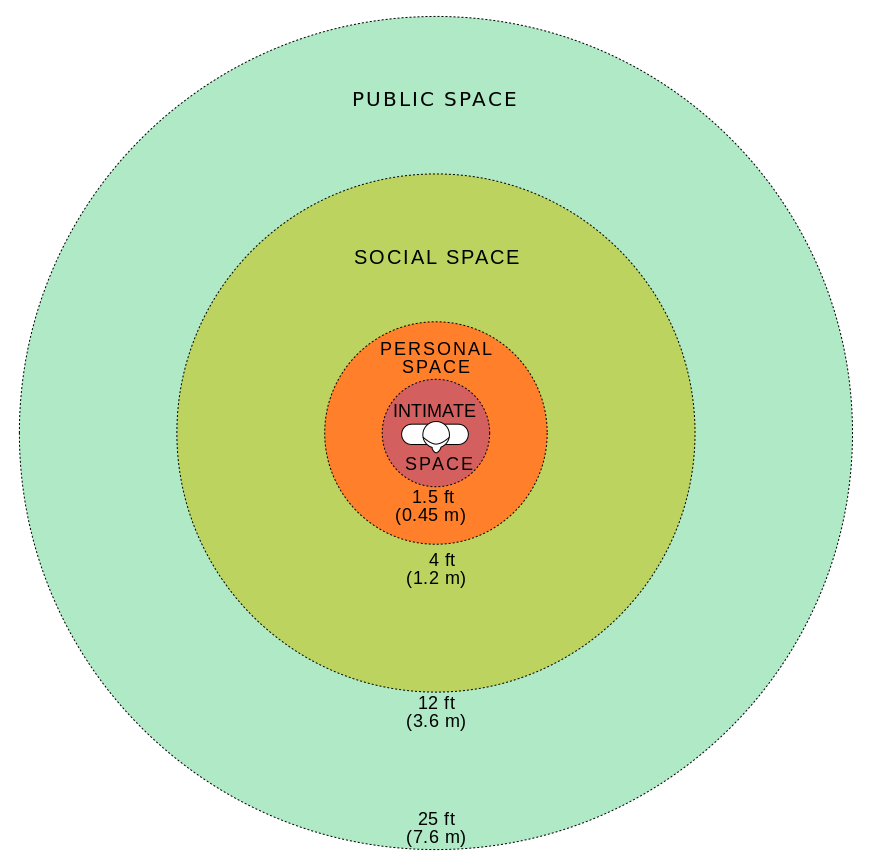
\includegraphics[width=0.6\textwidth]{gfx/882px-Personal_Space.png}
	\caption{Przedstawienie stref zaproponowanych przez E.T. Halla w metrach i stopach\cite{dimension_zones}}
	\label{fig:hall_zones}
\end{figure}

Badania dotyczące stref społecznych mają istotny wkład w kwestii naturalności ruchu robota. Robot pracujący z człowiekiem musi przestrzegać odległości, zależnie od wykonywanych zadań i (prawdopodobnie) konstrukcji robota. Strefy personalne implementowane najczęściej za pomocą pól potencjału, bądź pewnych funkcji kosztu \cite{survey}. Drugie podejście obrazuję rysunek \ref{fig:cost_zones}. Podobną koncepcje można również wykorzystać w przypadku proszujacego się człowieka, gdzie kształt strefy personalnej, na bazie wektora ruchu, można obliczyć przy pomocy funkcji gaussowskich\cite{nrs}. Część badaczy wysuwa jednak wniosek, że istotniejszym czynnikiem niż przestrzeganie dystansu, jest przestrzeganie zasad społecznych, kulturowych. To ich naruszenie powoduje dyskomfort pracy z robotem \cite{survey}\cite{survey_2}. Wskazaną umiejętnością robota jest także redukowanie prędkości przy podejściu do człowieka, oraz zachowanie odpowiedniego kierunku skierowania sensorów, jeżeli robot, w jakimś stopniu, posiada budowę humanoidalną.

\begin{figure}[H]
	\centering
	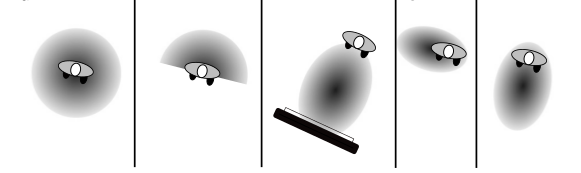
\includegraphics[width=0.7\textwidth]{gfx/cost_zone.png}
	\caption{Rysunki przedstawiają przykładowe strefy o zwiększonym koszcie ruchu wokół człowieka. Mogą się one różnić w zależności od przyjętych założeń lub kontekstu\cite{survey}}
	\label{fig:cost_zones}
\end{figure}

Kwestia nawigacji i unikania kolizji robot-człowiek nie byłaby możliwa bez rozwiązania problemu planowania trajektorii ruchu. Opracowane na przestrzeni lat algorytmy przedstawia rysunek \ref{fig:taxonomy}.

\begin{figure}[H]
	\centering
	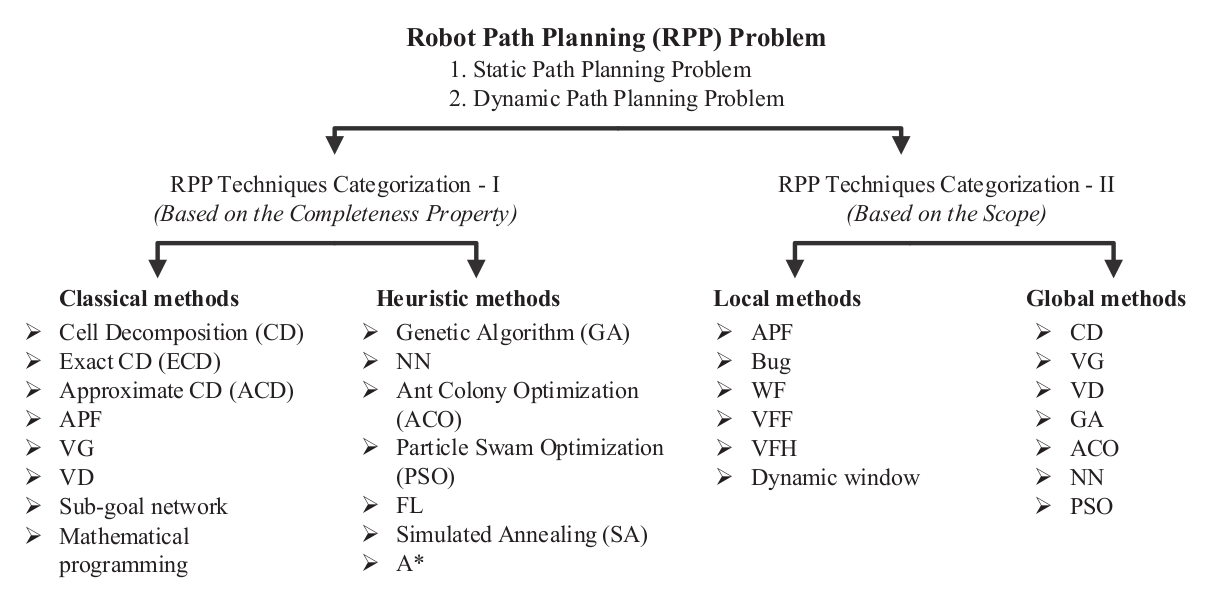
\includegraphics[width=0.9\textwidth]{gfx/taksonomia_planery.png}
	\caption{Taksonomia algorytmów planowania ścieżki dla robotów mobilnych\cite{taxonomy}}
	\label{fig:taxonomy}
\end{figure}

Algorytmy planowania ścieżki można podzielić na metody klasyczne i heurystyczne. Celem metod klasycznych jest wyznacznie najlepszej możliwej ścieżki, bądź stwierdzenie, że takowa nie istnieje. Odbywa się to jednak kosztem dużego nakładu obliczeniowego. Algorytmy heurystyczne nie gwarantują znalezienia ani optymalnego rozwiązania, ani znalezienia rozwiązania w ogóle \cite{planer_1}. Zaletą algorytmów heurystycznych jest jednak większa szybkość działania. Algorytmy można podzielić również na metody globalne i lokalne. Globalne odnoszą się do pewnego zbioru danych na temat przeszkód w środowisku, które znane jest a priori, nie są one jednak efektywne w przypadku ruchomych przeszkód. Do tego celu wykorzystuje się metody lokalne, które operują na danych dostarczonych przez receptory, takie jak kamery RGB czy skanery laserowe \cite{taxonomy}\cite{planer_1}\cite{planer_2}. Metody lokalne nie są jednak odpowiednie do wyznaczenia globalnej ścieżki ruchu ze względu na możliwość niepowodzenia generacji ścieżki. Często więc systemy planowania trajektorii ruchu budowane są z użyciem dwóch planistów, globalnego, który wyznacza ogólną ścieżkę ruchu od robota do zadanego celu i lokalnego, którego zadaniem jest obliczenie aktualnego wycinka ścieżki \cite{taxonomy}. \\

Kompletnym systemem realizującym zadania nawigacji w środowisku człowieka jest system opracowany przez E.A. Sisbota, L.F Marina-Uriasa, R. Alami i T. Simeona w 2007, opisany w pracy {\textit{A Human Aware Mobile Roobt Motion Planner}}\cite{ma}. Praca zakładała stworzenie planisty ruchu uwzględniającego pozycje, posturę (siedząca, stojąca) oraz zależności przestrzennych takich jak nie przejeżdzanie w niewielkiej odległości od człowieka, tuż za jego plecami, czy też bliskość przeszkód blokujących pole widzenia danej osoby. Architektura planisty znajduję się na rysunku \ref{fig:hamp_arch}.


\begin{figure}[H]
	\centering
	\subcaptionbox{Architektura modułu HAMP \cite{ma} \label{fig:hamp_arch}}[0.4\linewidth]{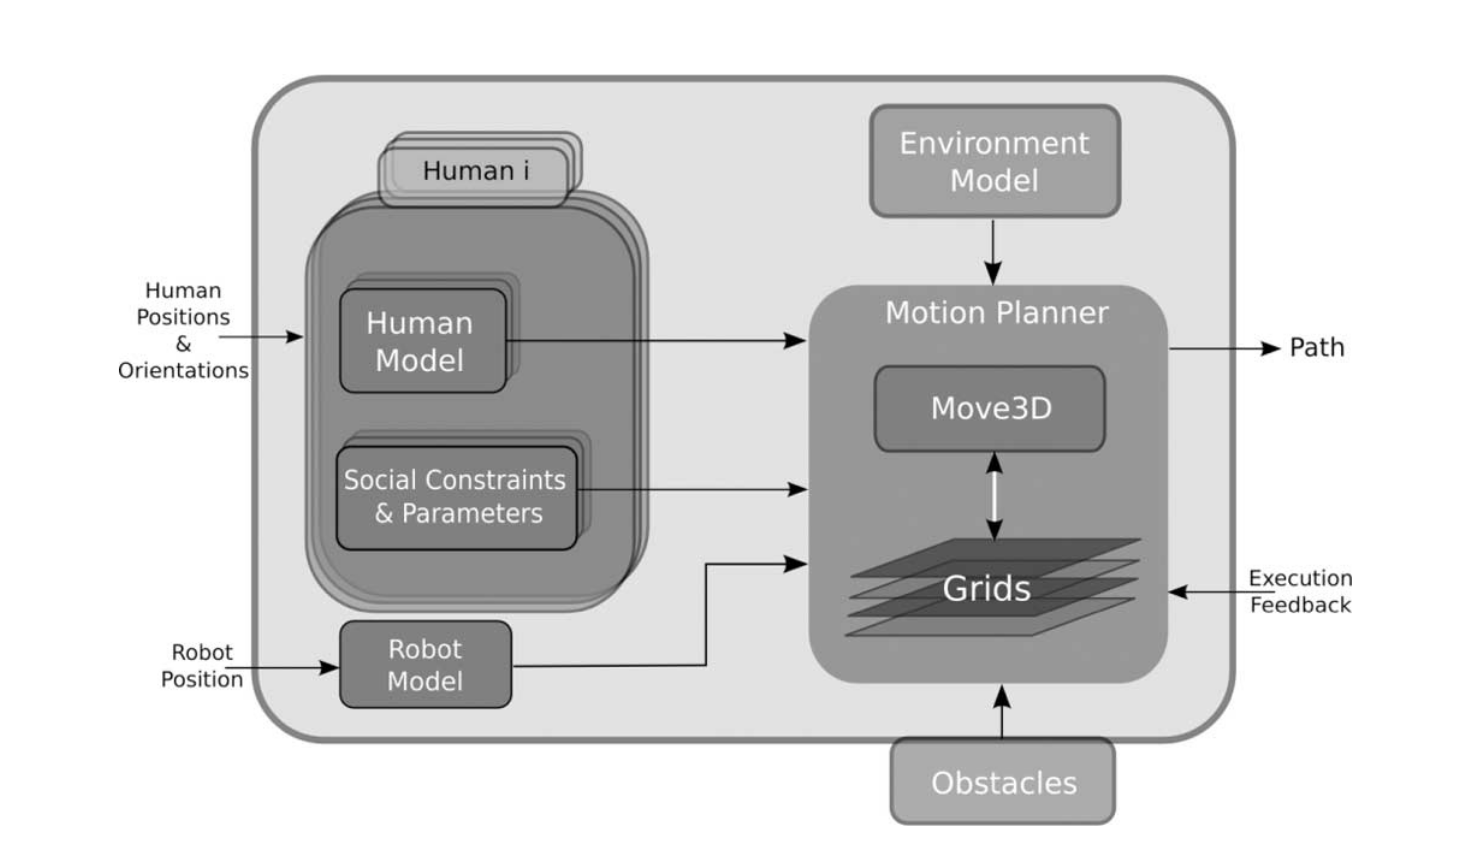
\includegraphics[height=4.25cm]{gfx/HAMP_arch.png}}		
	\subcaptionbox{Architektura modułu systemu detekcji ludzi \cite{ma} \label{fig:hamp_detector}}[0.4\linewidth]{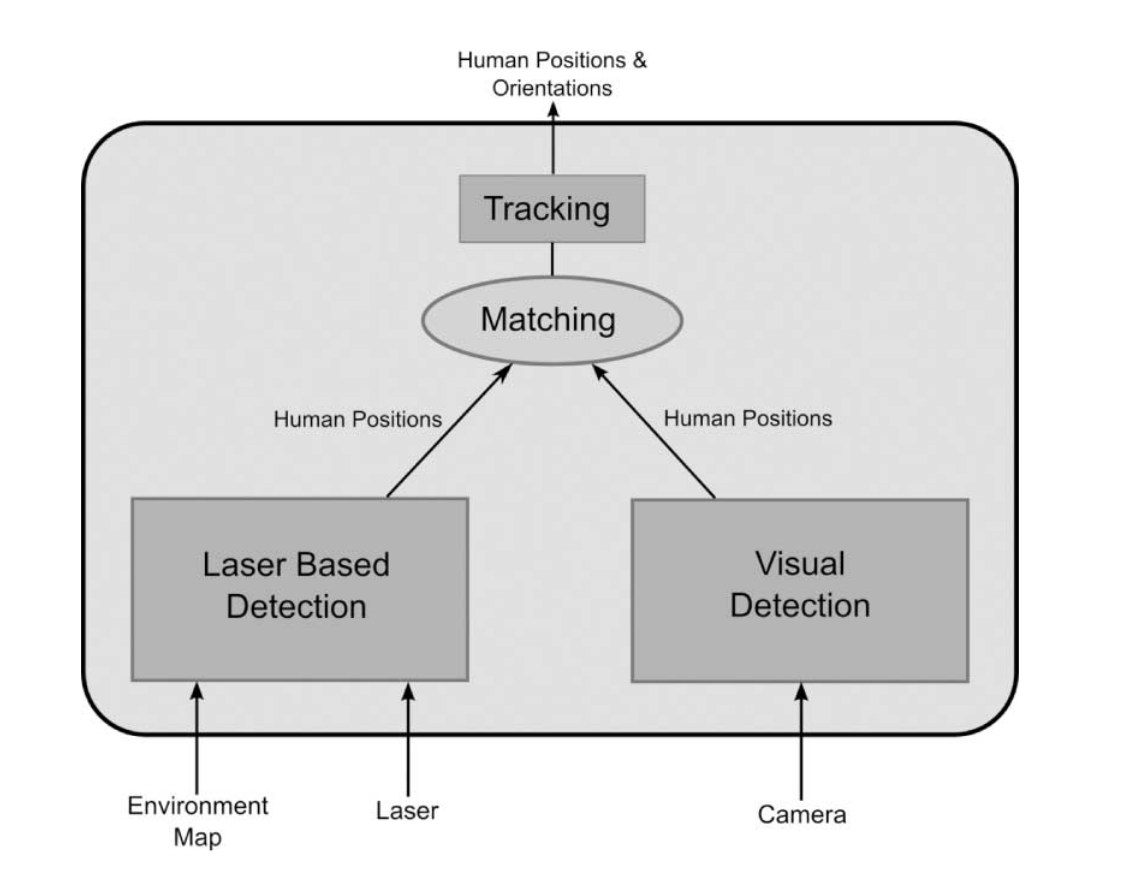
\includegraphics[height=4.25cm]{gfx/HAMP_detector.png}}		
	\caption{Architektura systemu}
	\label{fig:hamp_main}
\end{figure}


Niezależnie od modułu planisty zaimplementowano również system wykrywania człowieka na bazie odczytów sensorów laserowych oraz kamery RGB. Dane pozyskane z sensorów laserowych były przetwarzane przez algorytm pozwalający na wykrycie nóg człowieka. Na tej podstawie można było stwierdzieć jego położenie. Obraz z kamery RGB służył do detekcji twarzy z bliskiej odległości. Wykryte osoby były następnie śledzone przez robota. Architektura systemu detekcji znajduję się na rysunku \ref{fig:hamp_detector}.

Badacze sformułowali dwa kryteria: bezpieczeństwa - zapewniające bezpieczeństwo człowiekowi i robotowi, poprzez zapewnienie odpowiedniego dystansu oraz widoczności - stwierdzono, że ludzie czują się lepiej, gdy robot znajduję się w ich polu widzenia. Koszt łączny bezpieczeństwa i widoczności \ref{eq:cost_1}, był następnie nanoszony na mapę kosztu, z której korzystał zaimplementowany planista ruchu.


\begin{figure}[h!t]
  	\centering 
  	\begin{equation} \label{eq:cost_1}
  	Cost_{merged}(x,y) = w_{1}Cost_{safety}(x,y) + w_{2}Cost_{visibility}(x,y)
  	\end{equation}   
  	\capequation{Wzór kosztu łącznego zastosowany w systemie, $x$ i $y$ to współrzędne na mapie, a $w_{1}$ i $w_{2}$ to współczynniki wagowe.} 
\end{figure}
    
    
    
